\chapter{含风电电力系统的脆弱性量化分析}
\label{cha:quantiAnaly}

\section{引言}
\label{sec:index5}
依据本文所建立的含风电电力系统脆弱性分析方法,对系统进行脆弱性分析评估。首先根据系统的特性进行建模,包括随机性风电功率模型与随机性负荷概率模型。其次针对系统的拓扑和状态进行脆弱性分析,得到系统的脆弱性指标集。最后分别采用层次分析法和$D-S$证据理论对二级指标和一级指标进行融合,最终得到系统的综合脆弱性。

本章以$IEEE39$电力系统为例,在系统模型建立的基础上,分别研究了单风机接入和多风机接入下系统的脆弱性。单风机接入的情况下,研究了系统的结构脆弱性,并且对比了不同风机接入下系统的状态脆弱性,最终得到单风机系统的综合脆弱性。多风机接入的情况下,首先对比了双风机与单风机系统的脆弱性,再对多风机系统的脆弱性进行分析。最后,使用不同的电力系统数据进行脆弱性量化分析。
\section{$IEEE39$风力发电系统的模型}
\label{sec:modelIntroduce}
鉴于真实的电力系统结构过于庞大、复杂,且具体的拓扑及数据参数属于保密范畴,因此本文选择新英格兰测试系统数据$\raisebox{0.5mm}{------}$一套广泛用于学术研究的数据系统作为研究对象,进行脆弱性分析与量化评估。这套数据按照节点数目的不同而具有不同的测试数据集。

本节采用$IEEE39$测试系统进行仿真实验,首先对$IEEE39$测试系统的组成进行一个简单的介绍。该系统由10个发电节点,29个负荷节点和46条传输线路组成。该系统的基准电压为345$KV$,基准功率为100$MVA$。其中负荷节点则被称为$PQ$节点,即负荷节点的有功功率和无功功率已知,待求的是电压幅值和相角。由表\ref{tab:chap5:load39}所示,节点序号从1到29。

发电节点又被称为$PV$节点,即发电节点的有功功率和节点电压已知,待求的是无功功率和电压相角。由表~\ref{tab:chap5:generator39}~所示,节点序号从30到39,其中31节点为平衡节点。平衡节点的作用是提供系统的相位基准,这样系统中其他节点的电压相位以它为参考,由于该节点为$V\Theta$节点,对系统起到功率平衡的作用。
\begin{table}[H]
   \centering
   \caption{$IEEE$39系统负荷节点}
   \label{tab:chap5:load39}
     \begin{tabular}{C{1.2cm}C{2.4cm}C{2.4cm}C{1.2cm}C{2.4cm}C{2.4cm}}
\toprule
             \textbf{节点名}        &\textbf{额定有功功率($MW$)}      &\textbf{额定无功功率($MVar$)}   & \textbf{节点名}        &\textbf{额定有功功率($MW$)}      &\textbf{额定无功功率($MVar$)}       \\
\midrule
             1        &97.6 &44.2 & 16        &329.0 &32.3\\
             2        &0.0 &0.0 &17        &0.0 &0.0\\
             3        &322.0  &2.4 &18        &158.0 &30.0\\
             4        &500.0  &184.0 &19        &0.0 &0.0\\
             5        &0.0 &0.0 &20        &680.0 &103.0\\
             6       &0.0 &0.0 &21        &274.0 &115.0\\
             7        &233.8 &84.0 &22        &0.0 &0.0\\
             8        &522.0 &176.6 &23        &247.5 &84.6\\
             9        &6.5 &-66.6 &24        &308.6 &-92.2\\
             10        &0.0 &0.0 &25        &224 &47.2\\
             11        &0.0 &0.0 &26        &139 &17\\
             12        &8.53 &88.0 &27        &281 &75.5\\
             13        &0.0 &0.0 &28        &206 &27.6\\
             14        &0.0 &0.0 &29        &283.5 &26.9\\
             15        &320.0 &153.0 & & &\\
\bottomrule
\end{tabular}
\end{table}

\begin{table}[H]
   \centering
   \caption{$IEEE$39系统发电节点}
   \label{tab:chap5:generator39}
     \begin{tabular}{C{3cm}C{3cm}C{3cm}}
\toprule
 \textbf{节点名}        &\textbf{额定有功功率($MW$)}      &\textbf{是否为平衡节点}         \\
\midrule
             30        &250 &否\\
             31        &677.81 &是 \\
             32        &650  &否 \\
             33        &632  &否 \\
             34        &508   &否\\
             35        &650 &否\\
             36        &560 &否\\
             37        &540 &否\\
             38        &830 &否\\
             39        &1000 &否\\
\bottomrule
\end{tabular}
\end{table}

由第二章的研究可知,本文采用韦伯分布表示风速的概率模型如式~\ref{equ:chap2:Index3}~,式中的$P_R$为对应的发电机节点的额定有功功率,额定风速为15$m/s$,切入风速为5$m/s$,切出风速为20$m/s$。负荷变化采用正态分布的概率模型如式~\ref{equ:chap2:Index4}~,其中均值为对应负荷节点的额定功率,标准差为对应的额定功率的$0.2$倍,根据正态分布的特性可知,随机负荷的功率$95.449\%$分布在两个标准差的范围内(0.8倍到1.2倍之间)。至此,$IEEE39$风力发电系统的模型建立完毕。

\section{单风机电力系统脆弱性分析评估}
\label{sec:singleAssessment}
根据本文之前的研究内容,这一节对含单个风机的电力系统的脆弱性进行了分析。以$IEEE39$测试系统为例,分别将不同位置的发电节点接入风能,通过分析系统的结构脆弱性和状态脆弱性得到系统的综合脆弱性指标,在此基础上得出相应的结论。

\subsection{单风机电力系统结构脆弱性分析}
\label{sec:singleAnalysis_fabric}
由前文可知,系统的结构脆弱性表征的是当意外发生时,系统自身组成因素遭到破坏后仍能够保持结构完整的能力。因此,通过拓扑的不同建模,我们得到了基于复杂网络的无向图模型和基于$PageRank$的有向图模型,分别得到了各自对应的系统结构脆弱性指标。再将这三个二级指标进行融合,得到系统的结构脆弱性指标。

首先针对$IEEE39$系统的结构特点,可以得到如下的拓扑示意图。
\begin{figure}[H] % use float package if you want it here
  \centering
  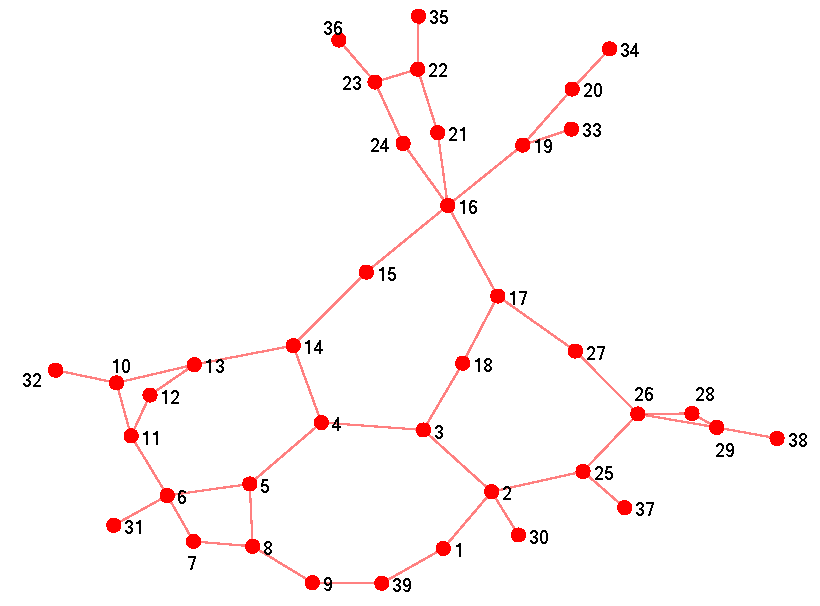
\includegraphics[height=8.3cm]{fabric_39.pdf}
  \caption{IEEE39系统拓扑示意图}
  \label{fig:fabric_39}
\end{figure}

由于结构脆弱性指标的实质反映的是节点在拓扑中的重要程度,因此结构脆弱性指标的归一化选择了排序归一法,即按照节点在拓扑中的重要性排序进行量化。重要性最小的节点脆弱性指标为0,重要性最大的节点脆弱性指标为1。用这种方法量化了各自的二级指标后,再根据层级分析法得出的权重向量$W(1)=\left[~0.2599~~0.4126~~0.3275~\right]$进行融合得到结构脆弱性指标。如下表所示,由于每个结构脆弱性二级指标表示的意义不同所以计算的结果不同。在39个节点中,电气度指标最大的是节点6,电气介数指标最大的是节点16,$PR$排序指标最大的是节点4。

\begin{table}[H]
\centering
\caption{IEEE39~系统结构脆弱性指标}
\label{tab:chap5:Index_frabric39}
\begin{tabular}{C{1.5cm}C{2.75cm}C{2.75cm}C{2.75cm}C{2.75cm}}
\toprule
\textbf{节点序号} & \textbf{电气度指标} & \textbf{电气介数指标} & \textbf{PR排序指标} & \textbf{结构脆弱性指标} \\
\midrule
1  & 0.105263158 & 0.131578947 & 0.447368421 & 0.228160526 \\
2  & 0.815789474 & 0.973684211 & 0.684210526 & 0.837844737 \\
3  & 0.289473684 & 0.947368421 & 0.921052632 & 0.767763158 \\
4  & 0.394736842 & 0.473684211 & 1           & 0.625534211 \\
5  & 0.842105263 & 0.105263158 & 0.631578947 & 0.469136842 \\
6  & 1           & 0.421052632 & 0.710526316 & 0.666323684 \\
7  & 0.578947368 & 0.236842105 & 0.526315789 & 0.420557895 \\
8  & 0.657894737 & 0.5         & 0.815789474 & 0.644457895 \\
9  & 0.052631579 & 0.394736842 & 0.868421053 & 0.460955263 \\
10 & 0.894736842 & 0.763157895 & 0.421052632 & 0.685315789 \\
11 & 0.684210526 & 0.368421053 & 0.289473684 & 0.424639474 \\
12 & 0           & 0           & 0.236842105 & 0.077565789 \\
13 & 0.605263158 & 0.184210526 & 0.263157895 & 0.319497368 \\
14 & 0.447368421 & 0.157894737 & 0.578947368 & 0.371023684 \\
15 & 0.184210526 & 0.289473684 & 0.842105263 & 0.443102632 \\
16 & 0.973684211 & 1           & 0.947368421 & 0.975923684 \\
17 & 0.236842105 & 0.078947368 & 0.763157895 & 0.344063158 \\
18 & 0.078947368 & 0.052631579 & 0.736842105 & 0.28355     \\
19 & 0.868421053 & 0.657894737 & 0.394736842 & 0.626426316 \\
20 & 0.631578947 & 0.868421053 & 0.552631579 & 0.703444737 \\
21 & 0.763157895 & 0.526315789 & 0.605263158 & 0.613726316 \\
22 & 0.921052632 & 0.736842105 & 0.368421053 & 0.664060526 \\
23 & 0.789473684 & 0.894736842 & 0.473684211 & 0.729484211 \\
24 & 0.210526316 & 0.315789474 & 0.657894737 & 0.400471053 \\
25 & 0.736842105 & 0.578947368 & 0.315789474 & 0.5338      \\
26 & 0.526315789 & 0.342105263 & 0.789473684 & 0.536494737 \\
27 & 0.157894737 & 0.263157895 & 0.894736842 & 0.442642105 \\
28 & 0.263157895 & 0.210526316 & 0.5         & 0.319007895 \\
29 & 0.947368421 & 0.684210526 & 0.342105263 & 0.640565789 \\
30 & 0.131578947 & 0.447368421 & 0           & 0.218781579 \\
31 & 0.552631579 & 0.026315789 & 0.026315789 & 0.163105263 \\
32 & 0.473684211 & 0.789473684 & 0.052631579 & 0.466084211 \\
33 & 0.421052632 & 0.710526316 & 0.078947368 & 0.42845     \\
34 & 0.315789474 & 0.552631579 & 0.105263158 & 0.344563158 \\
35 & 0.5         & 0.815789474 & 0.131578947 & 0.509636842 \\
36 & 0.368421053 & 0.631578947 & 0.157894737 & 0.408052632 \\
37 & 0.342105263 & 0.605263158 & 0.184210526 & 0.398973684 \\
38 & 0.710526316 & 0.842105263 & 0.210526316 & 0.601065789 \\
39 & 0.026315789 & 0.921052632 & 0.973684211 & 0.705747368 \\
\bottomrule
\end{tabular}
\end{table}

根据计算可以得到系统的结构脆弱性结果如下图。由图可知,该系统的拓扑中重要程度最高的节点是16,由拓扑示意图不难看出,该节点位于拓扑的中心位置,且与该节点相连的支路有5条,这些支路承担了较多的能量输送,负责把位于拓扑边缘的发电节点产生的电能输送至各负荷节点,所以该节点对拓扑的重要性大。其次重要性较高的节点分别是2、3、23、39,这些节点无论是从复杂网络模型的角度还是从$PageRank$模型的角度而言都是对整个拓扑非常重要的节点。同时,不难看出计算结果中结构脆弱性较低的节点有12、31、30、1,这些节点由于自身在拓扑中所起的作用小,所连支路的传输力小所以具有较小的重要性。
\begin{figure}[H] % use float package if you want it here
  \centering
  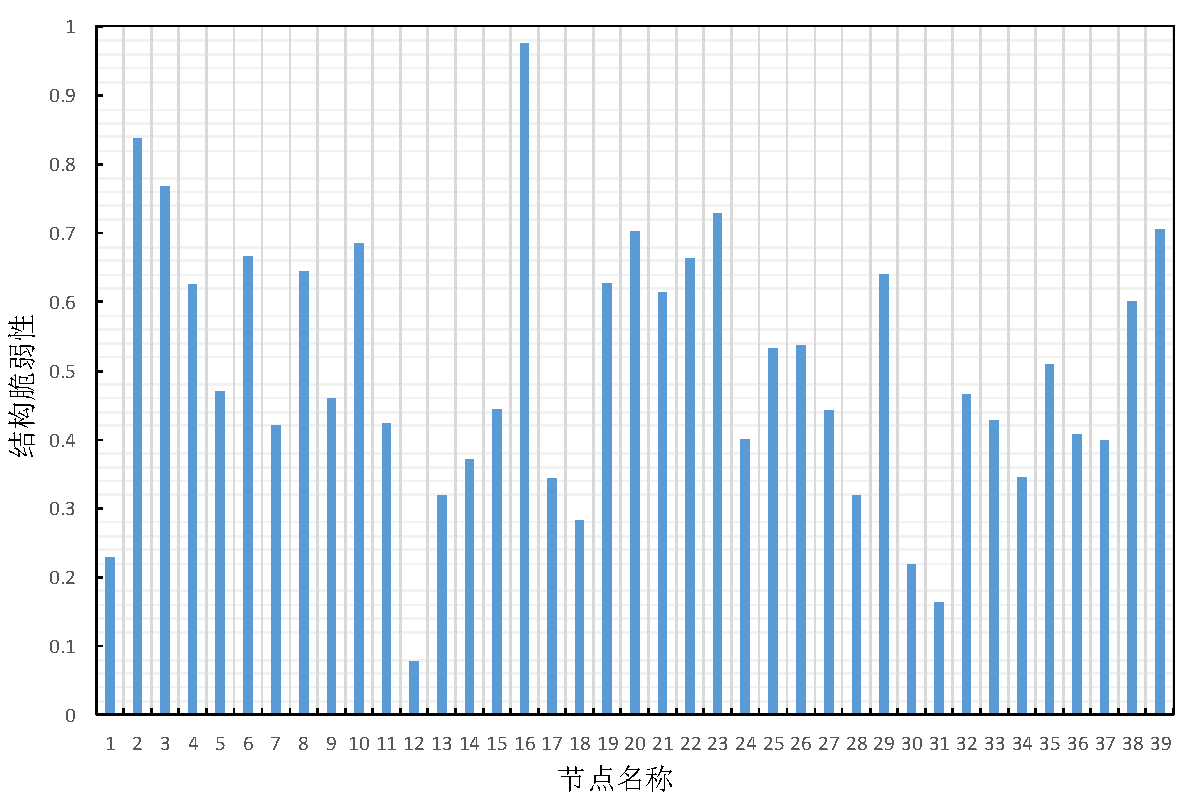
\includegraphics[height=9.9cm]{39fabric_histogram.pdf}
  \caption{IEEE39系统结构脆弱性结果}
  \label{fig:39fabric_histogram}
\end{figure}

\subsection{单风机电力系统状态脆弱性分析}
\label{sec:singleAnalysis_status}
本节研究单个风机接入时系统的状态脆弱性,鉴于$IEEE39$系统的发电节点有10个,从节点30到节点39,因此分别研究每个发电节点被风机代替后对整个系统的影响。根据之前的研究可知,含风电系统的状态脆弱性使用蒙特卡洛的方法通过大量的实验模拟随机性风速和负荷的作用下系统各节点电压偏差的状态。由于发电节点在潮流计算中是$PV$节点,即节点的功率和电压固定为已知量,所以理论上发电节点在环境变化中,其电压状态不发生改变。因此,系统状态脆弱性的评估分析只针对负荷节点,对于$IEEE39$系统而言,即从节点1到节点29。

下图表示的是发电节点39接入风电后,系统所有负荷节点状态脆弱性的变化。其中,指标1代表的是环境变化过程中,各负荷节点的电压越线率,在接入39风机后,导致不同负荷节点的越线率差异很大。指标2代表的是负荷节点电压偏差的期望,在环境的变化过程中,该指标的变化幅度较小。指标3代表了节点电压偏差的方差,整个变化中该指标数值较小,差异性不大。然后,根据层次分析法得到的权重向量$W(2)=\left[~0.5396~~0.2970~~0.1634~\right]$进行指标融合,进一步得到状态脆弱性指标。
\begin{figure}[H] % use float package if you want it here
  \centering
  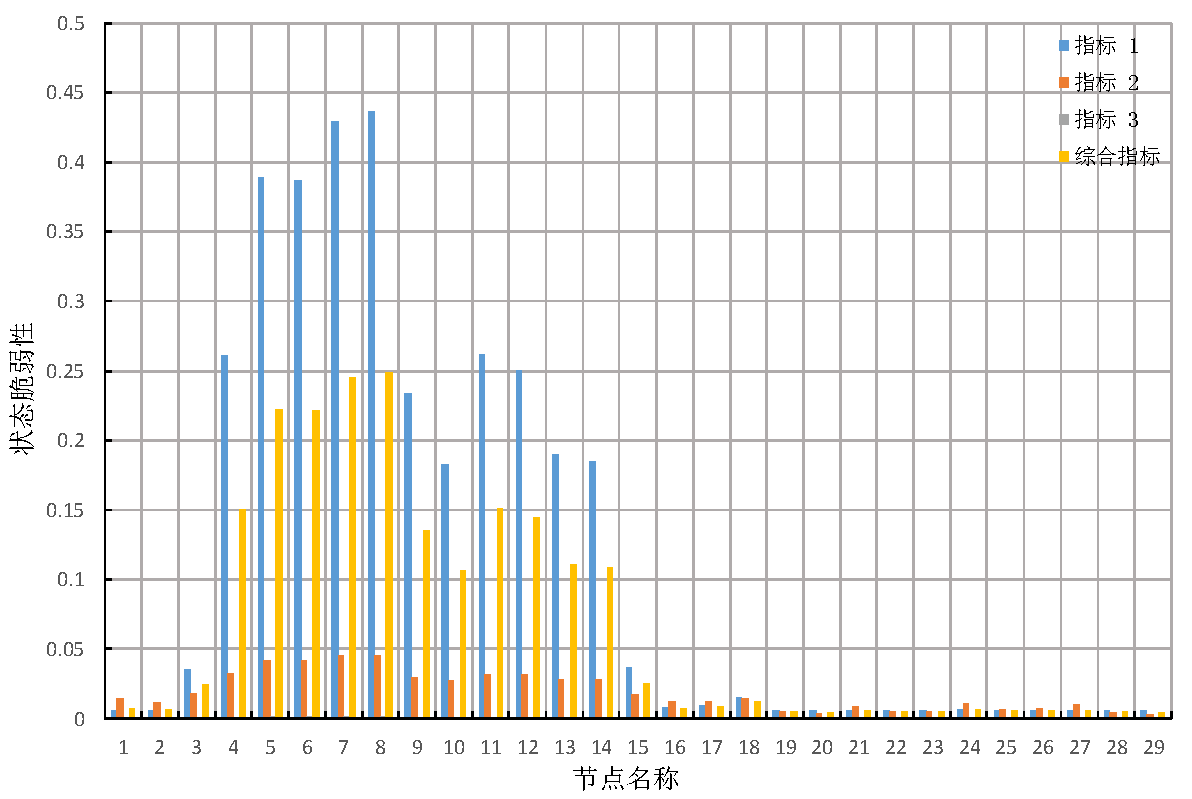
\includegraphics[height=9.9cm]{singleVuln_status_alload_gen10.pdf}
  \caption{发电节点39接入风电对负荷节点状态脆弱性影响}
  \label{fig:singleVulnLoadGen10}
\end{figure}

以节点5的状态脆弱性为观察对象,对比了不同发电节点被风机代替后,其状态脆弱性指标的变化,如下图。由图可见,接入单个风机的不同导致同一个负荷节点的脆弱性指标的变化也不同。其中,指标1在接入单个风机不同的情况下,该指标变化剧烈。指标2的变化幅度较小,指标3在整个变化中本身数值就很小,变化较平。

图\ref{fig:singleWindForLoad5}表示的是不同单风机接入下同一个负荷节点的状态脆弱性的变化。图中结果显示,在$IEEE39$系统中,当39、38发电机被风机代替后,对负荷节点5的影响比较大。由该系统的组成不难看出,发电节点39的输出功率1000$MW$是所有发电节点中功率最大的,发电节点39的输出功率830$MW$其次最大,其他发电节点的功率较小。由于这两个发电节点本身的输出功率远超其他发电节点,所以它们各自接入风能对系统状态的影响最大,体现在节点电压的越线率、节点电压偏差的期望都很大。这也是使负荷节点5状态脆弱性指标在后期发生较大幅度变化的原因。
\begin{figure}[H] % use float package if you want it here
  \centering
  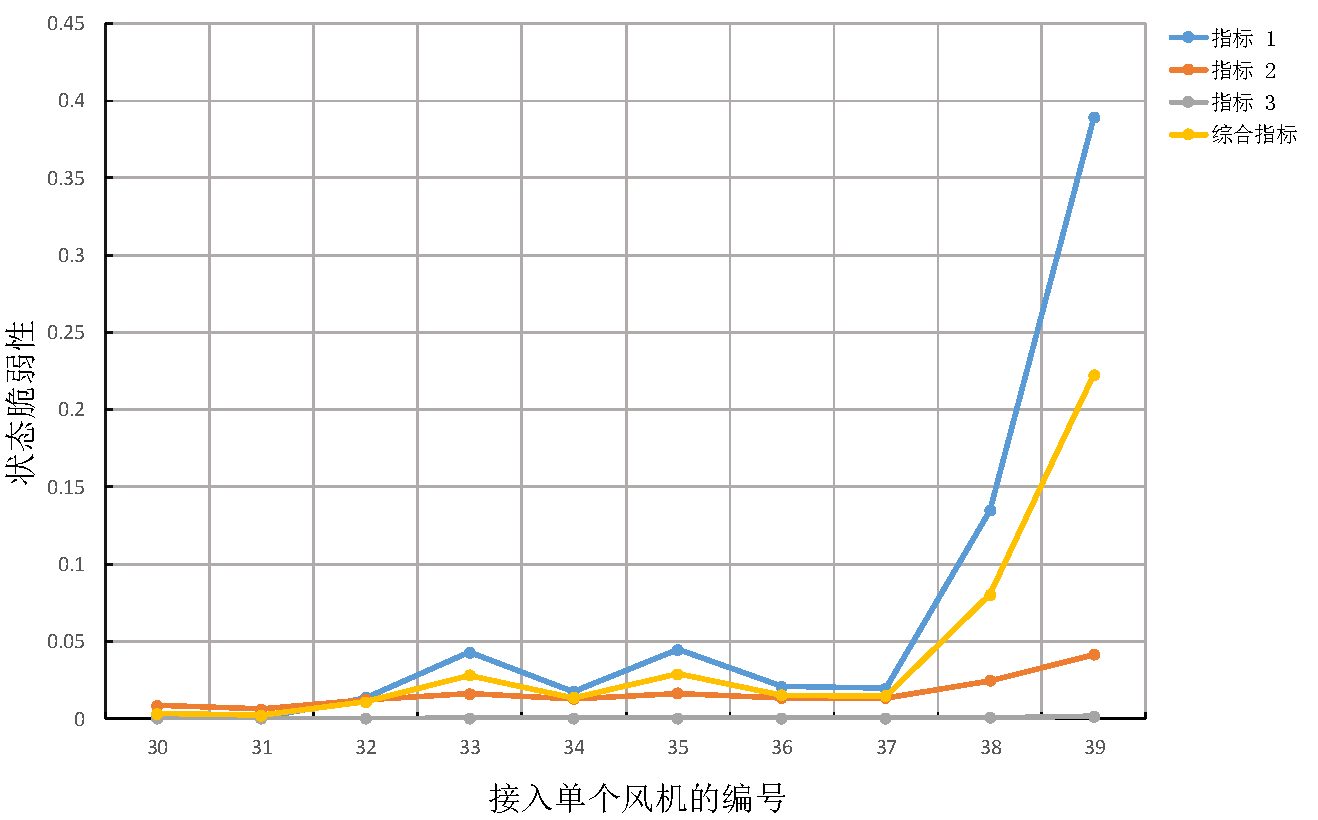
\includegraphics[height=8.58cm]{singleWindForLoad5.pdf}
  \caption{不同风机接入对负荷节点5的状态脆弱性影响}
  \label{fig:singleWindForLoad5}
\end{figure}
然而对于拥有着相同输出功率的发电机节点如32和35,其额定输出功率都是650$MW$,上述结果显示它们各自接入风能对同一负荷节点的影响是不同的。于是对比了这两个相同功率的单风机接入下系统的状态脆弱性如图\ref{fig:singleVuln_status_similarP},结果表明35接入风电对负荷节点的影响比32接入风电的影响普遍较大。
\begin{figure}[H] % use float package if you want it here
  \centering
  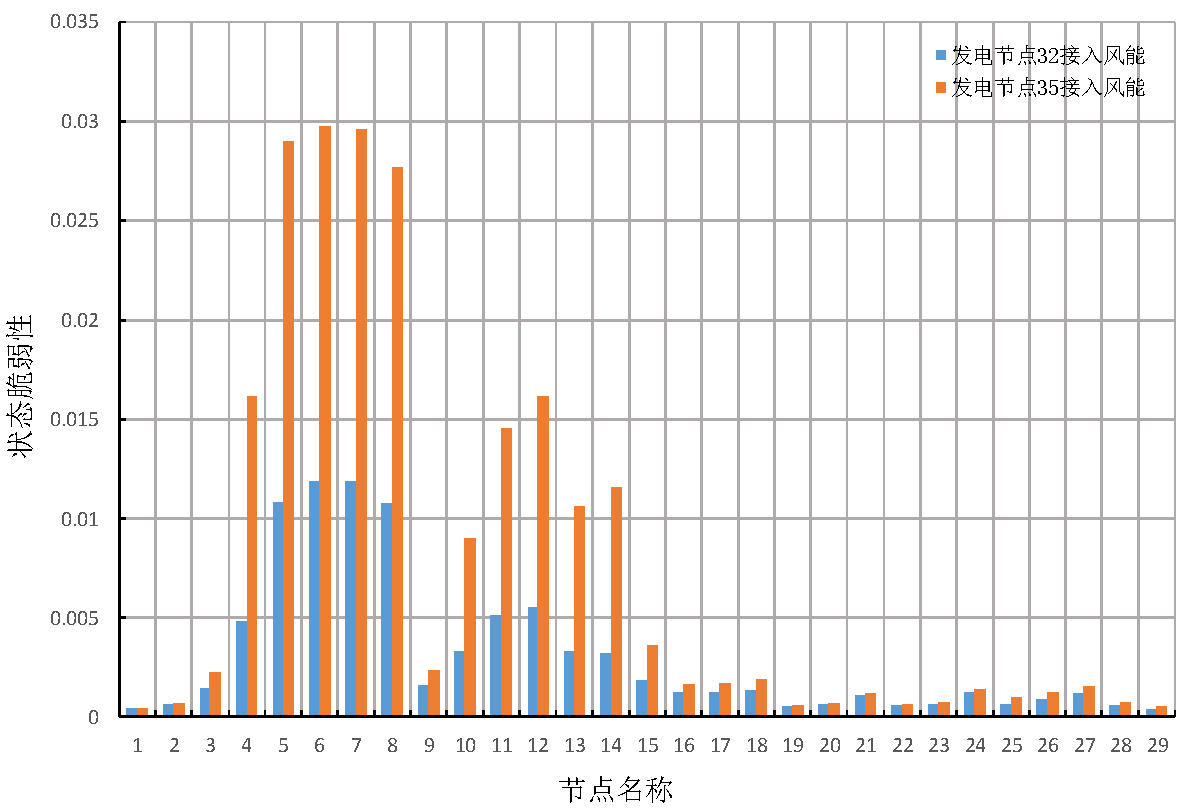
\includegraphics[height=9.5cm]{singleVuln_status_similarP.pdf}
  \caption{相同功率的单风机接入下系统的状态脆弱性}
  \label{fig:singleVuln_status_similarP}
\end{figure}

\subsection{单风机电力系统综合脆弱性分析}
\label{sec:singleAnalysis}
通过上面对单风机电力系统结构脆弱性分析与状态脆弱性分析,我们可以得到融合后的结构脆弱性指标与状态脆弱性指标,再根据4.4的$D-S$证据理论将这两个一级指标进行融合从而得到系统脆弱性的综合指标。由于系统的脆弱性分析主要针对负荷节点,所以本节的综合脆弱性的研究对象依然是$IEEE$39系统中的负荷节点1至负荷节点29。通过分析系统脆弱性综合指标,企图得到系统的薄弱环节。

下图显示的结果分别是发电节点依次单独接入风电后,系统各个负荷节点的综合脆弱性指标的变化。由于系统综合脆弱性指标融合了结构脆弱性指标与性能脆弱性指标,所以其计算结果会与上述得到的结果数值不同。但是我们发现,在不同的发电节点依次单独接入风电的情况下,负荷节点的脆弱性变化趋势却是大致相同的。也就是说脆弱性高的负荷节点无论是哪个发电节点单独接入风电它的脆弱性都相对较高,比如节点4、6、8、10、16。而脆弱性低的负荷节点在任何发电节点单独接入风电的情况下,其脆弱性都相对较小,比如节点1、19、20、22、28。
\begin{figure}[H] % use float package if you want it here
  \centering
  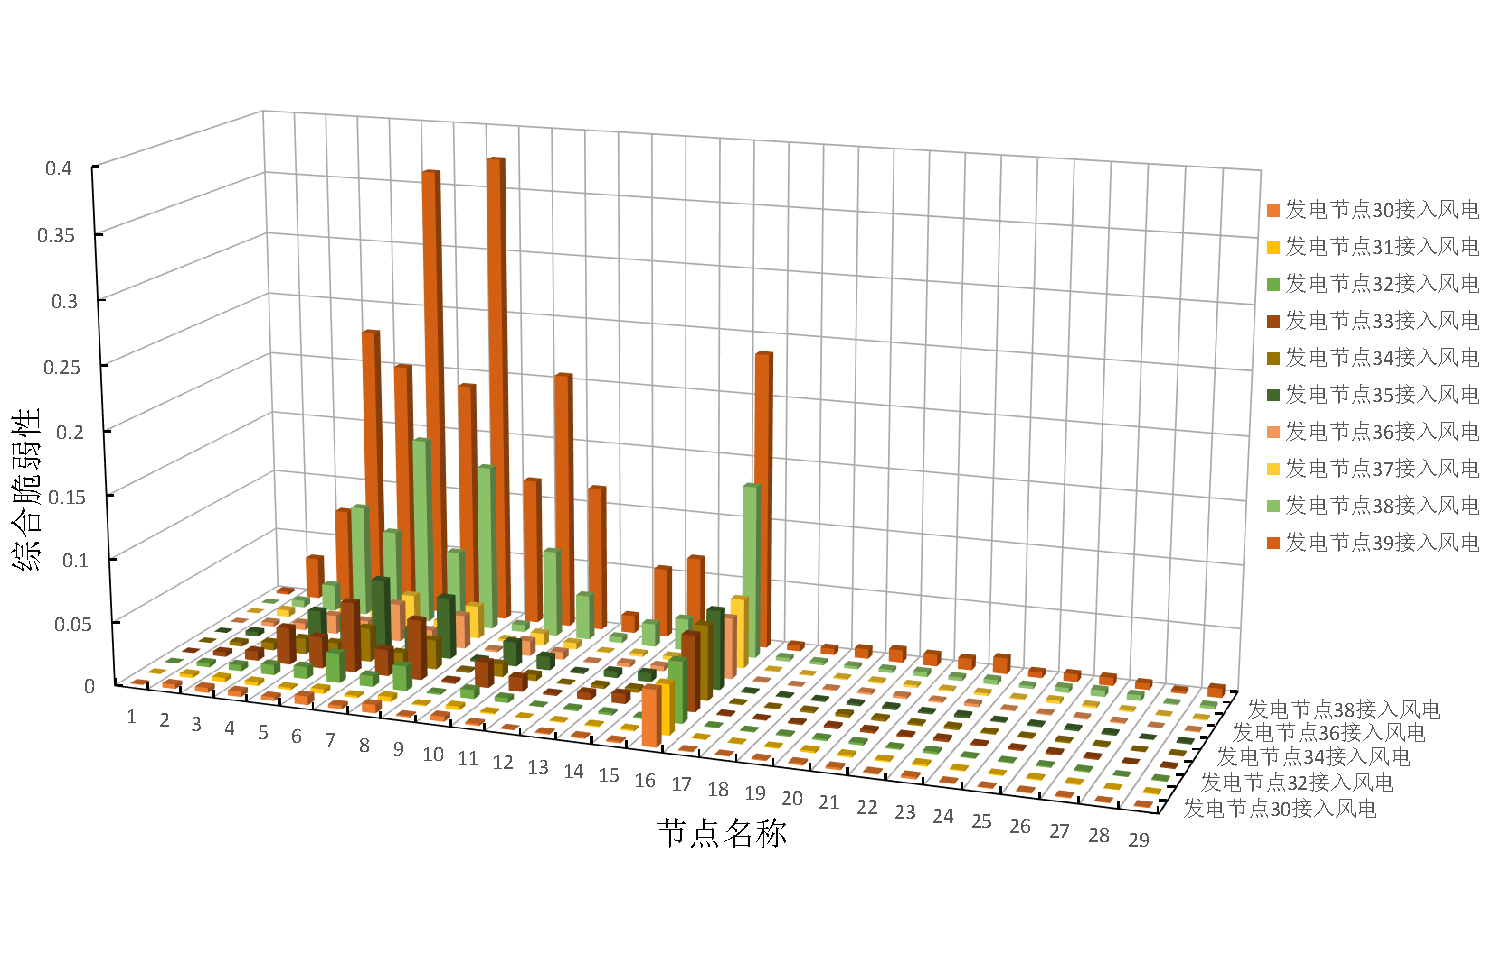
\includegraphics[height=9.7cm]{singleVuln_composite_39.pdf}
  \caption{单风机接入下负荷节点的综合脆弱性}
  \label{fig:singleVuln_composite_39}
\end{figure}

\section{多风机电力系统脆弱性分析评估}
\label{sec:multiAssessment}
上一节分析了单个风机接入下的系统脆弱性,本节着重对多个风机接入的电力系统的脆弱性进行研究,通过结构脆弱性指标和状态脆弱性指标进一步计算出系统的综合脆弱性。首先对比了双风机与单风机系统的脆弱性,再对多风机系统的脆弱性进行研究,从而得到一些有用的结论。

\subsection{双风机与单风机系统脆弱性比较}
\label{sec:multiVSsingle}
按照之前的分析,理论上两个风机接入会比单个风机接入使得系统的脆弱性变大,因为更多的风电接入使得系统的状态变化的不确定性更大,虽然结构脆弱性不会因此发生变化,但是随着状态脆弱性的变化使得系统的综合脆弱性变化很大。因此本节着重对比了双风机接入的电力系统的状态脆弱性与单风机接入的系统的状态脆弱性。

在$IEEE39$系统中,以32、33两个发电节点同时接入风电和各自分别单独接入风电为例,进行系统的脆弱性分析得到如下所示的结果。从图中可以看出,在双风机同时接入的情况下,原来脆弱性大的薄弱节点此时的脆弱性更大了。而对于同一个负荷节点而言,多一个发电节点接入风电会比任何发电节点单独接入风电的状态脆弱性都大。
\begin{figure}[H] % use float package if you want it here
  \centering
  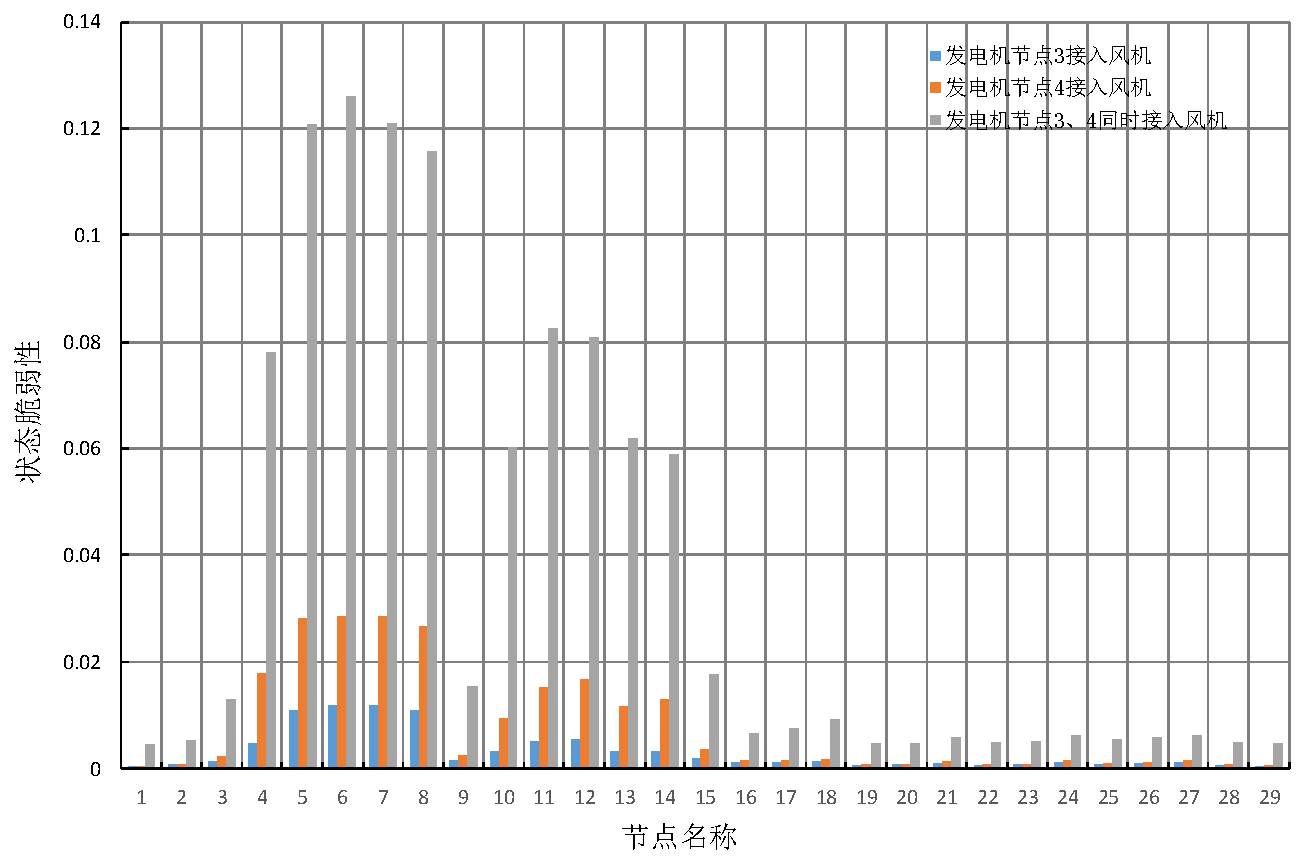
\includegraphics[height=9.5cm]{singleVSmulti_34.pdf}
  \caption{单风机与双风机接入下系统的状态脆弱性}
  \label{fig:singleVSmulti_34}
\end{figure}

\subsection{多风机电力系统脆弱性分析评估}
\label{sec:multiAnalysis}
在对比了双风机接入的电力系统后,本节对多风机接入的系统脆弱性进行研究。理论上由于更多数目的发电机节点被风机替代,使得系统状态变化的不确定性会更大。因此,本节通过不断地增加风机的数目来观察系统的脆弱性变化。

在$IEEE39$系统中,仿真实验起初是只有31发电节点接入风电,然后依次不断的增加接入风电的发电节点数目:32、32$\cdots$39,直到所有的发电节点都被接入风电。取负荷节点5作为研究对象,进行状态脆弱性分析得到如下的结果。由图可知,随着接入风机数目的增大,指标1增长迅速,到最后所有发电节都被风机取代后,指标1接近极大值1。这是因为由于越来越多的发电机被风机取代后,系统状态的随机性越来越大,使得系统处于脆弱域和不可运行域的几率越来越大。而当所有发电机都变成风机的时候,系统已经非常的脆弱了,几乎无法正常运行了。指标2和指标3虽然变化幅度较小,但是都在随着风机数目的增长而变大。最后得到的把三个指标融合的状态脆弱性指标也随着接入风机的数目在持续增长。可见风机的接入量直接影响着系统的状态脆弱性,且成正比的关系。
\begin{figure}[H] % use float package if you want it here
  \centering
  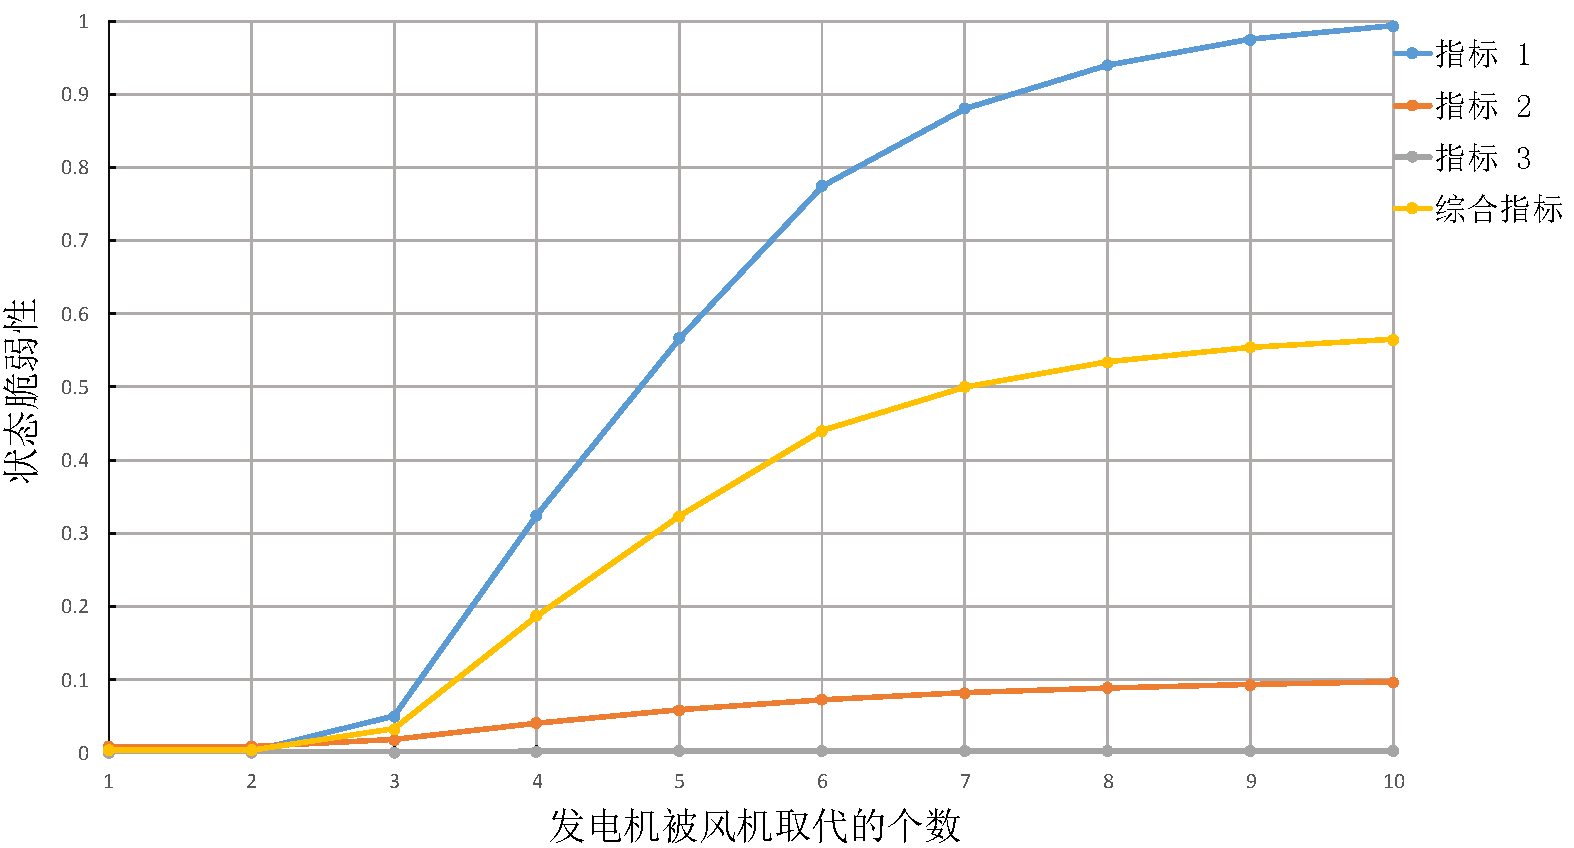
\includegraphics[height=8.0cm]{multiVuln_status_load5.pdf}
  \caption{风机接入数目对负荷节点5的状态脆弱性影响}
  \label{fig:multiVuln_status_load5}
\end{figure}

经过上述的研究分析,可知随着风机数目的增长负荷节点的状态脆弱性指标在逐渐增大,这表明系统的性能越来越差。通过结合状态脆弱性指标与结构脆弱性指标,我们可以得到随着接入风电的发电节点比率的增长,系统综合脆弱性的变化情况(如下图),从而找到系统的薄弱环节节点。从图中可以看出,随着风电接入量的增大,所有节点的脆弱性都有了不同程度的增长。其中一些脆弱性较高的节点在这个过程中一直保持远高于其他节点的脆弱性比如节点4、6、8、10、16。也有一些开始脆弱性相对较低的节点却逐渐增大称为脆弱性相对较高的节点,比如节点2、20、23,这都是系统拓扑和状态共同作用的结果。
\begin{figure}[H] % use float package if you want it here
  \centering
  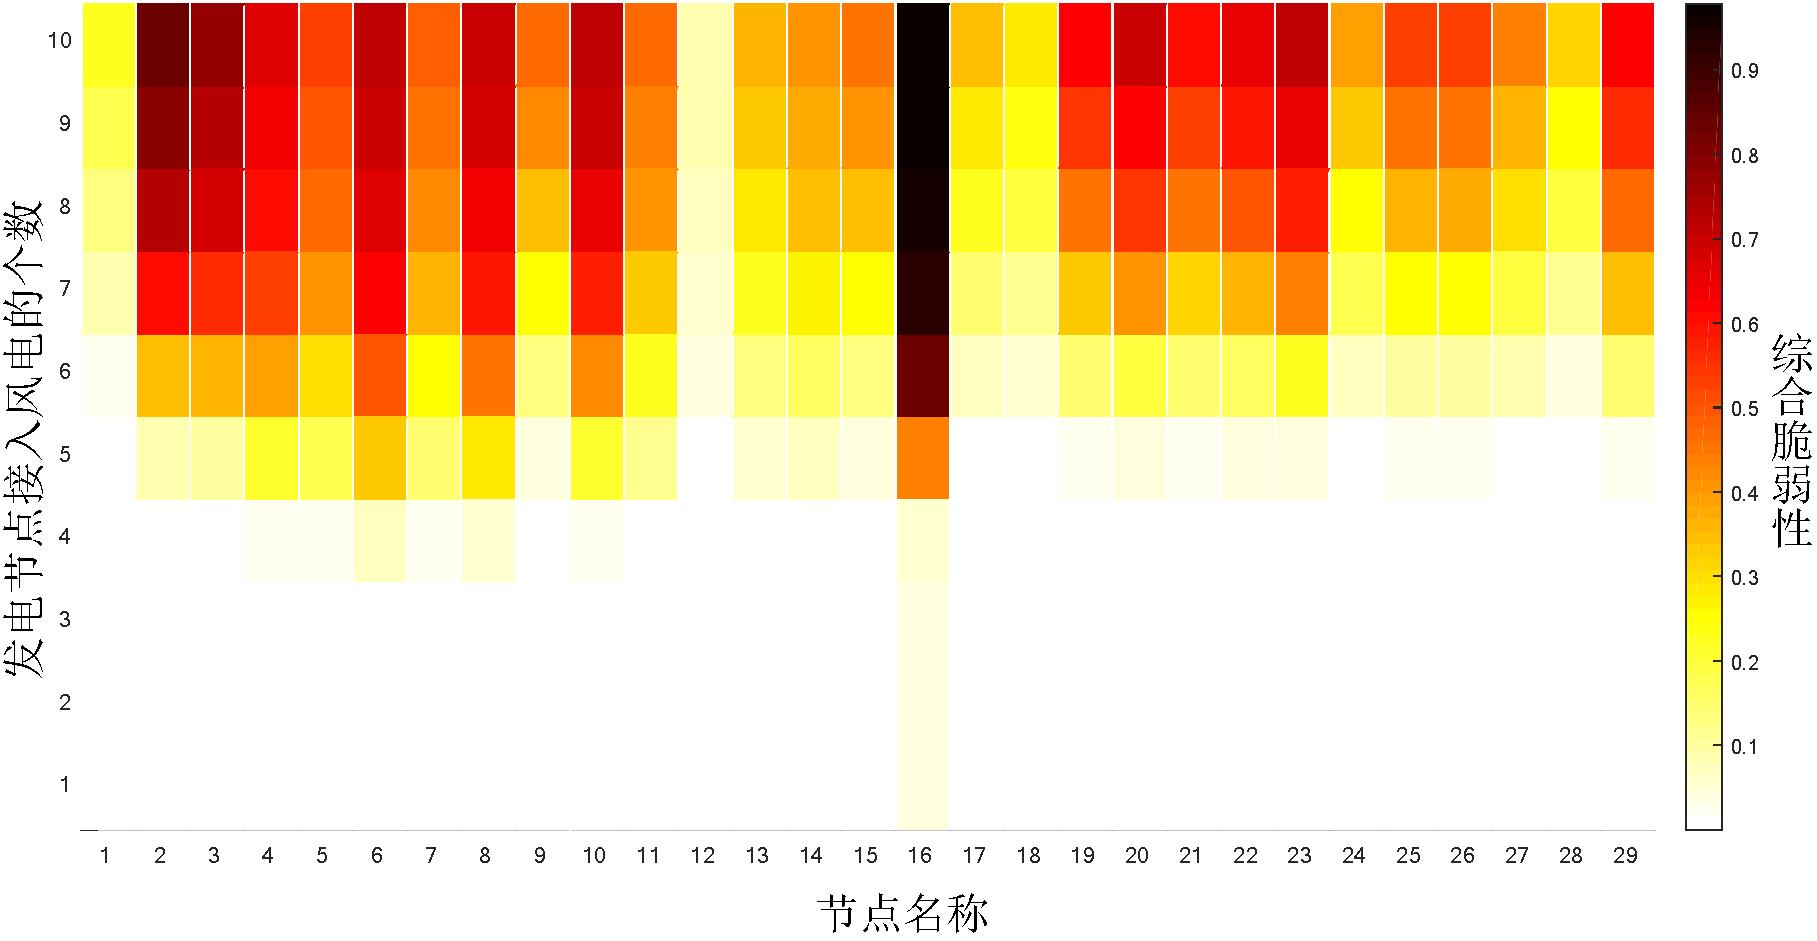
\includegraphics[height=7.6cm]{multiVuln_composite_39_3D.pdf}
  \caption{多风机接入下负荷节点的综合脆弱性}
  \label{fig:multiVuln_composite_39_3D}
\end{figure}

综合$IEEE39$系统在风电接入下的性能,包括单风机和多风机的情况。可以知道,该系统的风机数量大于4时,就会有负荷节点的脆弱性高于0.8,当风机数目大于6时,会有$24\%$的节点脆弱性高于0.5。所以系统的发电节点接入风电的量应该谨慎,越多系统越脆弱。考虑到单风机与多风机综合情况,认为该系统的薄弱节点有16、6、8、10、2、20、23等,这些节点对环境变化或意外的反应强烈,敏感度好,脆弱性大。相比之下,脆弱性较低的节点有1、12、24、28、18等,这些节点对环境变化具有较强的抵抗力,脆弱性小。
\section{其他风力发电系统的脆弱性分析}
\label{sec:otherSystemVuln}
为了验证本文所建立的含风电电力系统脆弱性分析方法具有普适性,本节对不同的数据系统进行了脆弱性分析。鉴于$IEEE118$是常用来实验研究的较大型的电力系统之一,所以选择该系统进行脆弱性分析。

\subsection{$IEEE118$风力发电系统的模型}
\label{sec:118model}
$IEEE118$测试系统具有118个节点,54个发电节点,64个负荷节点,186条支路。其拓扑示意图如下。该系统大多节点的基准电压为138$KV$,小部分节点的基准电压为345$KV$,基准功率为100$MVA$。具体的发电节点和负荷节点数据见附录$A$,从数据中可以看出发电节点中有很多节点的额定功率是0,只有19个发电节点额定有功功率不为0,所以随机性风电功率模型只能用在这些节点上。
\begin{figure}[H] % use float package if you want it here
  \centering
  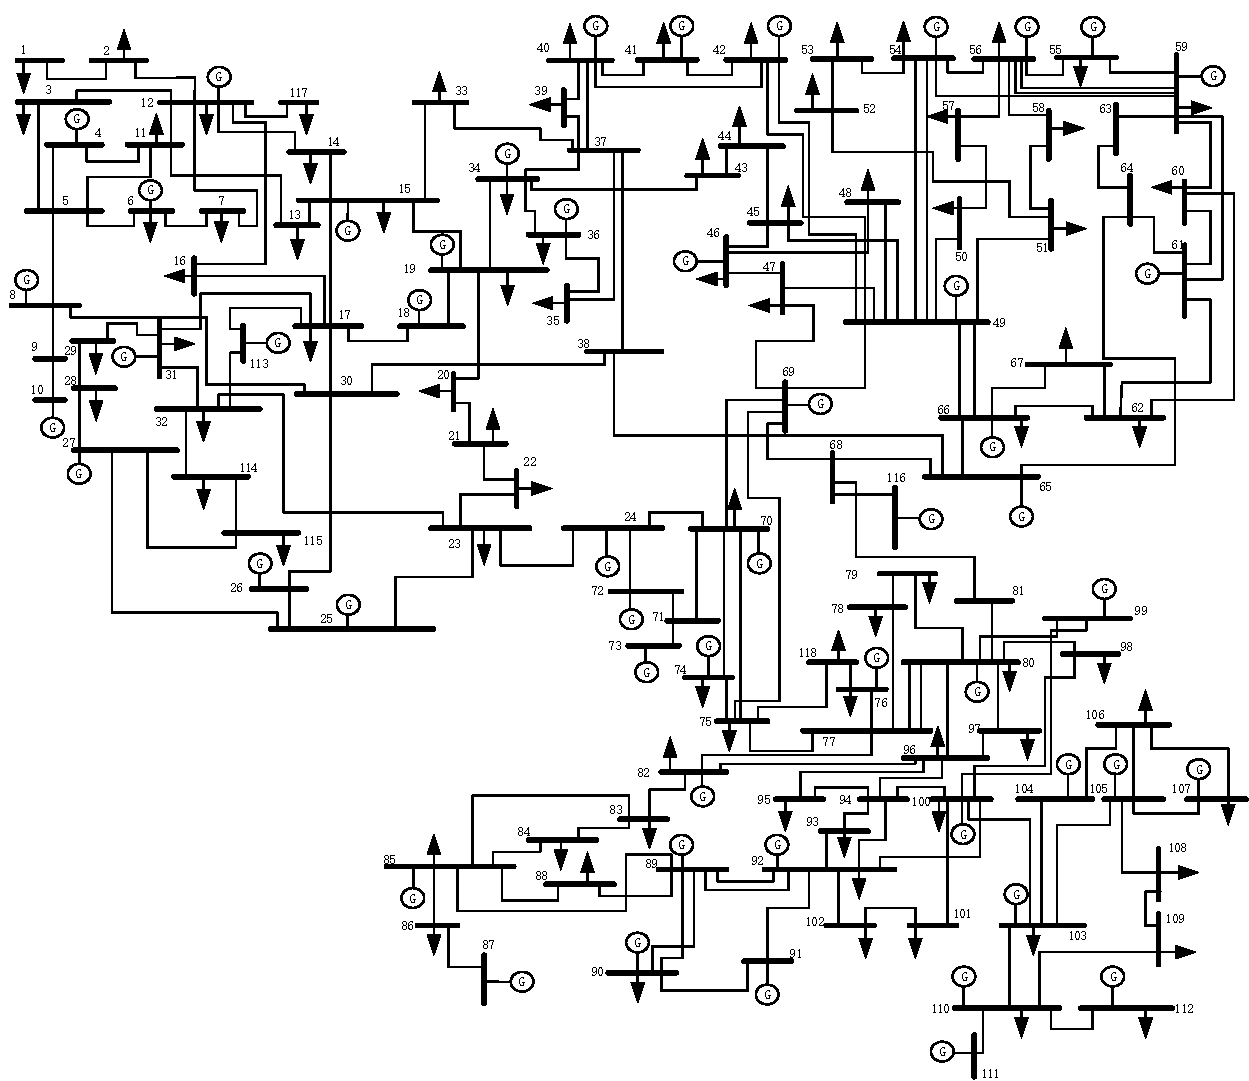
\includegraphics[height=10.8cm]{118model.pdf}
  \caption{$IEEE118$拓扑示意图}
  \label{fig:118model}
\end{figure}

该风力发电系统的建模依据第二章的研究,采用韦伯分布表示风速的概率模型,额定风速为15$m/s$,切入风速为5$m/s$,切出风速为20$m/s$。负荷变化采用正态分布的概率模型如式~\ref{equ:chap2:Index4}~,其中均值为对应负荷节点的额定功率,标准差为对应的额定功率的$0.2$倍,根据正态分布的特性可知,随机负荷的功率$95.449\%$分布在两个标准差的范围内(0.8倍到1.2倍之间)。至此,$IEEE118$风力发电系统的模型建立完毕。

\subsection{$IEEE118$系统脆弱性分析评估}
\label{sec:multiAnalysis118}
根据之前的研究理论,本节对$IEEE118$系统进行单风机电力系统脆弱性分析。首先根据结构脆弱性的定义,计算三个二级结构脆弱性指标,再将二级指标融合得到结构脆弱性指标。其次根据状态脆弱性的定义,研究不同的发电节点接入风电下系统状态的变化情况,得到状态脆弱性指标。最后根据$D-S$证据理论融合得到单风机系统的脆弱性。

下图为该系统的结构脆弱性指标结果,如图所示,该系统的拓扑重要程度较高的节点是100,77,59,5,8等,这些节点无论基于复杂网络模型还是$PageRank$模型都是非常重要的元素。相比之下,该系统的拓扑重要程度较低的节点是87、24、114、73、113等,这些节点在拓扑中的重要性相对较低。
\begin{figure}[H]
     \begin{adjustbox}{addcode={\begin{minipage}{\width}}{\caption{$IEEE$118系统结构脆弱性
         }\end{minipage}},rotate=-90,center}
         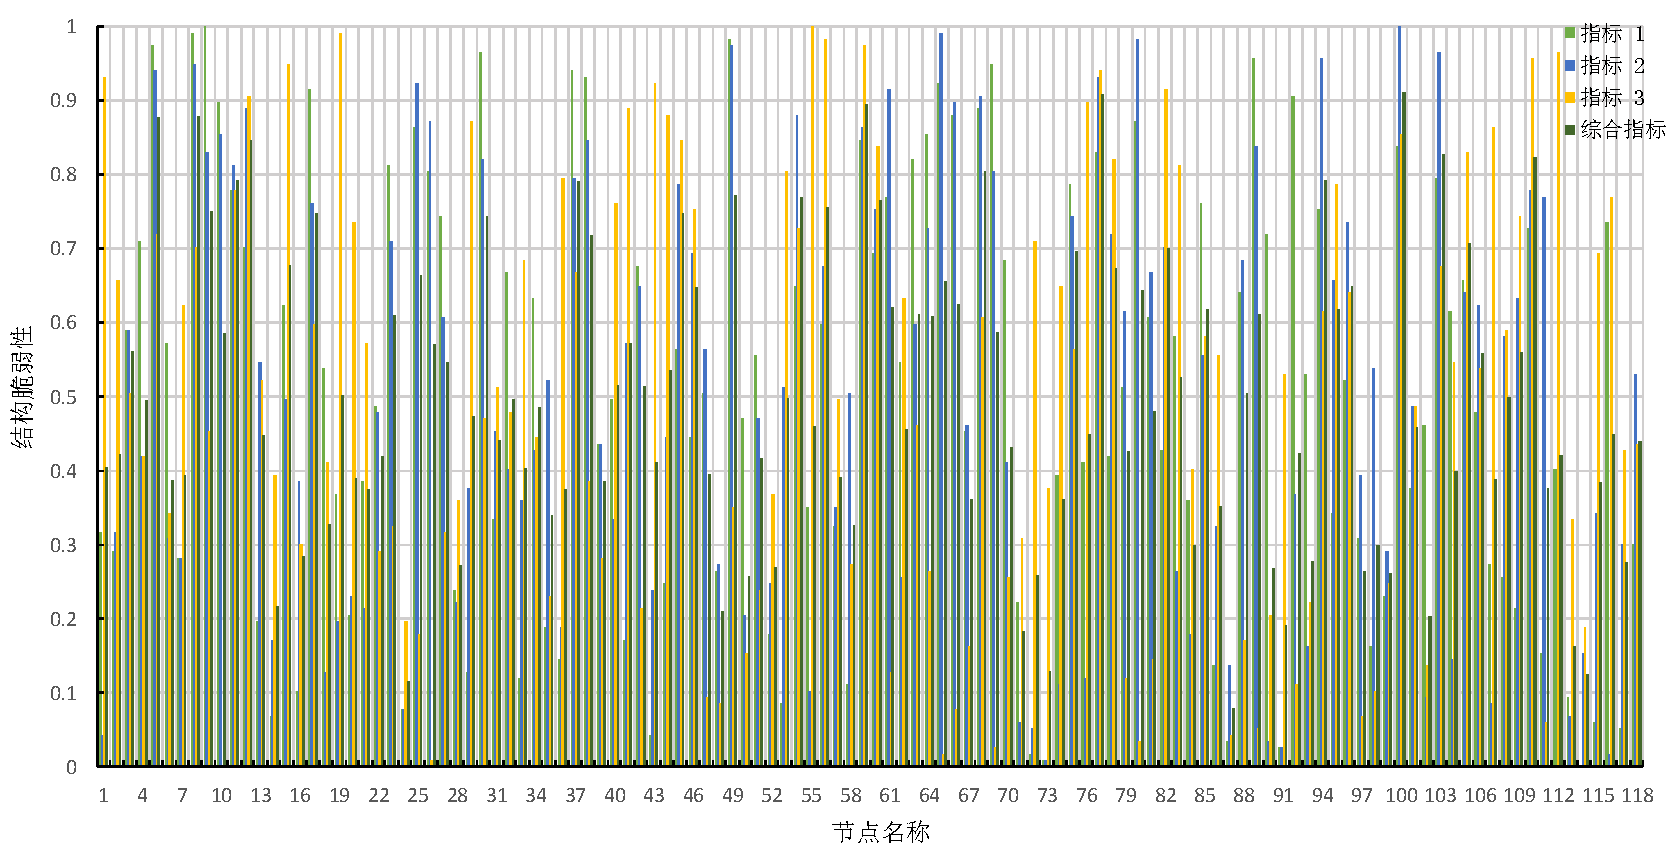
\includegraphics[height=12.5cm]{vuln_fabric_118.pdf}%
     \end{adjustbox}
\end{figure}

同样地,根据$IEEE118$系统的随机性风电功率模型和负荷概率模型进行蒙特卡洛实验统计得到系统的状态脆弱性指标。再根据$D-S$证据理论将系统的结构脆弱性指标和状态脆弱性指标进行融合得到系统的综合脆弱性指标。下表是发电节点10接入风电的单风机系统的脆弱性分析结果,由表可以看出,该单风机系统的脆弱性普遍偏小,这是因为该系统节点数目庞大,单个风机对系统状态的影响较小。其中,脆弱性较大的节点是节点9、节点30、节点38、节点45,这些节点即为该系统的薄弱环节。
\begin{table}[H]
\centering
\caption{$IEEE$118单风机电力系统负荷节点综合脆弱性}
\label{tab:chap5:generator118}
\begin{tabular}{C{1.4cm}C{2.2cm}C{1.4cm}C{2.2cm}C{1.4cm}C{2.2cm}}
\toprule
\textbf{节点名} & \textbf{综合脆弱性} & \textbf{节点名} & \textbf{综合脆弱性} & \textbf{节点名} & \textbf{综合脆弱性} \\
\midrule
2   & 0.000154385 & 41  & 0.000420636 & 82  & 0.001395726 \\
3   & 0.000266589 & 43  & 0.00163411  & 83  & 0.000543576 \\
5   & 0.000956597 & 44  & 0.003616794 & 84  & 0.000109745 \\
7   & 2.3506E-05  & 45  & 0.007050231 & 86  & 0.000245509 \\
9   & 0.302331265 & 47  & 0.000538372 & 88  & 0.000304921 \\
11  & 0.000819715 & 48  & 6.41342E-05 & 93  & 0.000112425 \\
13  & 0.000542244 & 50  & 7.41624E-05 & 94  & 0.001638393 \\
14  & 5.66768E-05 & 51  & 0.000321682 & 95  & 0.00131232  \\
16  & 0.000269775 & 52  & 0.000209298 & 96  & 0.000952485 \\
17  & 0.00181432  & 53  & 0.000626504 & 97  & 0.000127843 \\
20  & 0.000585624 & 57  & 0.000128436 & 98  & 0.000150473 \\
21  & 0.000817307 & 58  & 0.000148223 & 101 & 0.000471828 \\
22  & 0.00100946  & 60  & 0.000255372 & 102 & 5.15622E-05 \\
23  & 0.000886376 & 63  & 0.000109107 & 106 & 0.000494005 \\
28  & 8.38634E-05 & 64  & 9.83874E-05 & 108 & 7.44908E-05 \\
29  & 0.000123675 & 67  & 0.000136764 & 109 & 0.000124683 \\
30  & 0.005435762 & 68  & 9.52089E-05 & 114 & 2.17796E-05 \\
33  & 0.000591607 & 71  & 4.27656E-05 & 115 & 0.000106394 \\
35  & 7.21014E-05 & 75  & 0.001019156 & 117 & 0.000260899 \\
37  & 0.002718523 & 78  & 0.000454276 & 118 & 0.000301258 \\
38  & 0.009957741 & 79  & 0.00030221  &     &             \\
39  & 0.000203294 & 81  & 4.04024E-05 &     & \\
\bottomrule
\end{tabular}
\end{table}
此外,针对该系统的发电节点接入风电的数目不同的情况下,选取部分负荷节点的综合脆弱性指标的结果如下图。由图可以观察到,对于$IEEE118$这样的节点数目庞大的系统,随着风电接入数目的增大负荷节点的脆弱性虽然总体的趋势是增大的,但是并不完全成正相关的关系。而且由于该系统存在一大部分发电节点的有功功率输入为0,剩余的19个可接入风电的发电节点功率小且位置分散对负荷节点的影响普遍较小。所以相比之下,$IEEE39$风力发电系统的脆弱性结果变化起伏较大,而$IEEE118$风力发电系统实验结果符合结论但变化趋势略平缓。
\begin{figure}[H] % use float package if you want it here
  \centering
  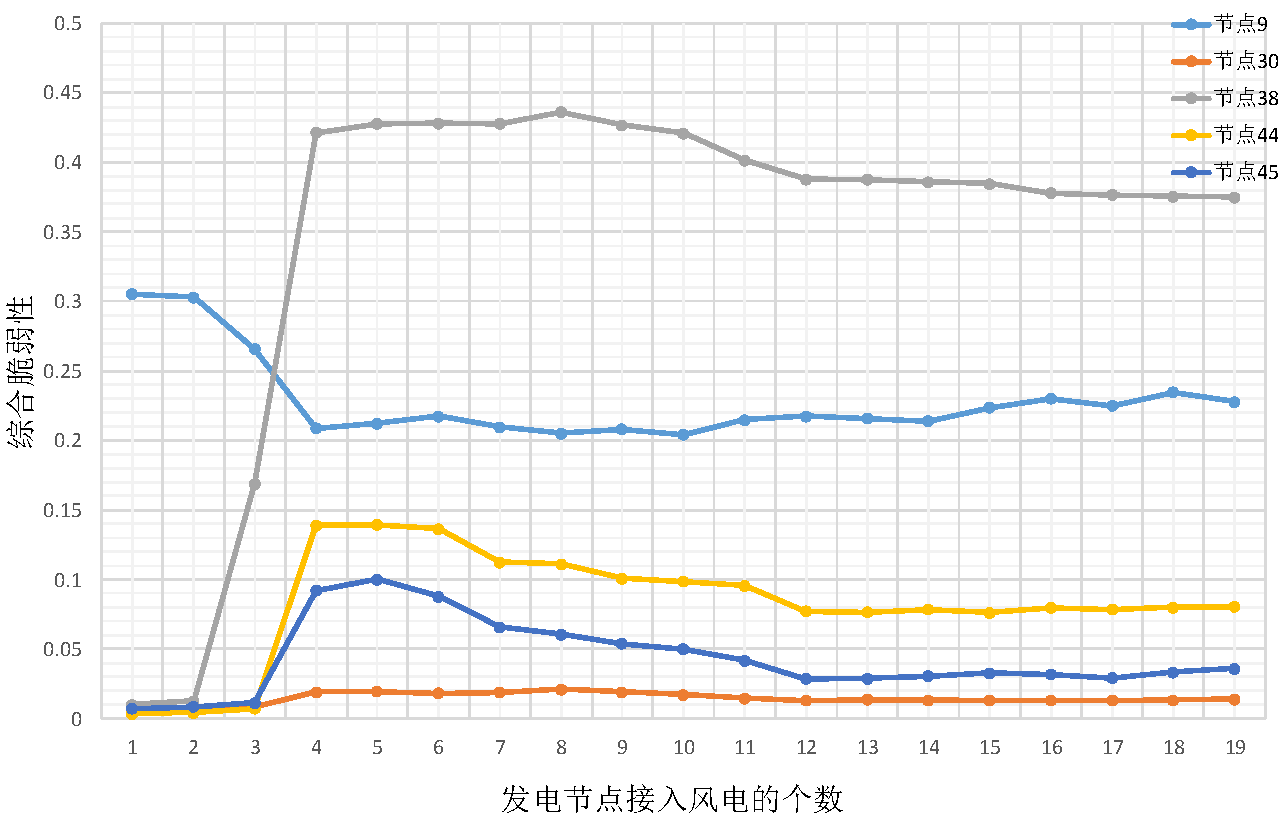
\includegraphics[height=9.4cm]{multiVuln_composite_118_partLoad.pdf}
  \caption{$IEEE$118多风机电力系统部分负荷节点的综合脆弱性}
  \label{fig:118model}
\end{figure}

\section{本章小结}
\label{sec:sum5}
本章以基于$IEEE39$风力发电系统作为研究对象,采用本文之前章节建立的脆弱性分析方法与量化评估模型进行脆弱性分析,详细地给出了脆弱性分析与量化评估的具体步骤。

依据前文对风力发电系统特性的研究分析,建立了随机性风电功率模型和负荷概率模型,模拟系统运行中外界环境及用户需求的随机性变化。借助$MATLAB$软件平台,根据第三章的理论对系统的结构脆弱性进行分析计算得到相应的指标,而状态脆弱性则分别针对单风机系统与多风机系统进行蒙特卡洛模拟实验进行统计得到相应的脆弱性指标。

根据分析计算出的各级指标,基于第四章建立的指标评估体系进行量化评估。首先将二级指标量化,再使用层次分析法进行融合得到一级指标。再使用$D-S$证据理论将两个一级指标融合得到系统的综合脆弱性。本章对$IEEE39$含风电电力系统脆弱性进行了详细的评估,此外,还使用$IEEE118$系统进行了补充评估验证。通过对系统脆弱性的评估得到对应系统的薄弱环节,对后续优化系统设计具有现实意义。

